\documentclass[11pt, letterpaper]{article}

% \usepackage[utf8]{inputenc}
% \usepackage[scaled]{helvet}
\usepackage[sfdefault]{inter}
\usepackage[T1]{fontenc}
\usepackage[utf8]{inputenc}
\usepackage{ctex}
\usepackage{geometry}
\geometry{left=2.2cm, right=2.2cm, top=2.5cm, bottom=2.5cm}
\usepackage{xcolor}
\usepackage{titlesec}
\usepackage{enumitem}
\usepackage{fancyhdr}
\usepackage{hyperref}
\usepackage[most]{tcolorbox}
\usepackage{amsmath, amssymb, amsthm}
\usepackage{physics}
\usepackage{braket}
\usepackage{helvet}
\usepackage{parskip}        % 自动处理段首不缩进和段间距
\usepackage{listings}
\usepackage{tikz}
\usetikzlibrary{positioning, arrows.meta}
\usepackage{subcaption}
\setlength{\parindent}{0pt} % 强制段首缩进为 0
\setlength{\parskip}{1em}
\renewcommand{\familydefault}{\sfdefault}

\hypersetup{colorlinks=true, linkcolor=blue, urlcolor=blue}

\definecolor{SBURed}{HTML}{990000} 
\definecolor{SoftGray}{HTML}{F4F4F4}
\definecolor{DeepGray}{HTML}{333333}

\usepackage{fontawesome5}

\newtcolorbox{referencebox}[1][]{title={\textcolor{white}{\faBook\ References}},
  colframe=RefBrown,
  colback=RefBeige,
  coltitle=black,
  fonttitle=\bfseries,
  arc=4pt,
  drop shadow,
  boxrule=2pt,
  breakable,
  left=10pt,right=10pt,top=8pt,bottom=8pt,
}


\hypersetup{
  pdfauthor={Zhehao Yi},   % Author of the document
  pdftitle={Quantum Computing: A Brief Introduction},   % Title of the document
  pdfsubject={Quantum Machine Learning}, % Subject of the document
  pdfkeywords={Tutorial},
  pdfcreator={Zhehao Yi}, % Creator
  pdfproducer={Zhehao Yi}, % PDF producer
  colorlinks=true,
  linkcolor=SBURed,
  urlcolor=SBURed,
  citecolor=SBURed
}

\tikzset{
    node_style/.style={
        circle,               % 节点形状为圆形
        draw=black,           % 边框颜色
        thick,                % 边框加粗
        fill=white,           % 填充颜色
        minimum size=8mm,     % 节点的最小尺寸
        font=\sffamily\large  % 节点文字字体
    },
    arrow_style/.style={
        -Stealth,             % 箭头形状 (Stealth 是一种比较现代的箭头)
        thick,                % 箭头线条加粗
        shorten >=1pt,        % 箭头终点稍微缩短，避免压到节点边框
        shorten <=1pt         % 箭头起点稍微缩短
    }
}

\pagestyle{fancy}
\fancyhf{}
\renewcommand{\headrulewidth}{0pt}
\fancyfoot[C]{\small \textcolor{gray}{\thepage}}
\fancyhead[L]{\small \textcolor{gray}{Zhehao Yi | Stony Brook University}}
\fancyhead[R]{\small \textcolor{SBURed}{Quantum Computing}}

\titleformat{\section}
  {\color{SBURed}\normalfont\Large\bfseries}
  {\thesection}{1em}{}[{\titlerule[0.8pt]}]

\titleformat{\subsection}
  {\color{DeepGray}\normalfont\large\bfseries}
  {\thesubsection}{1em}{}

\newtcolorbox{SBUBox}[1]{
    colback=gray!5!white,   % 浅灰色背景
    colframe=SBURed,        % SBU红边框
    coltitle=white,         % 标题文字白色
    fonttitle=\bfseries,    % 标题加粗
    title={#1},             % 传入标题
    sharp corners,          % 直角
    boxrule=1pt,            % 边框粗细
    toptitle=1mm,           % 标题内边距
    bottomtitle=1mm,
    left=2mm,               % 主体文字内边距
    right=2mm,
    before skip=15pt,       % 盒子前后的间距
    after skip=15pt
}

\definecolor{codegreen}{rgb}{0,0.6,0}
\definecolor{codegray}{rgb}{0.5,0.5,0.5}
\definecolor{codepurple}{rgb}{0.58,0,0.82}
\definecolor{backcolour}{rgb}{0.95,0.95,0.92}

\lstset{
    backgroundcolor=\color{backcolour},   
    commentstyle=\color{codegreen},
    keywordstyle=\color{magenta},
    numberstyle=\tiny\color{codegray},
    stringstyle=\color{codepurple},
    basicstyle=\ttfamily\small,          % 使用等宽字体
    breakatwhitespace=false,         
    breaklines=true,                     % 自动换行
    captionpos=b,                    
    keepspaces=true,                 
    numbers=left,                        % 行号在左侧
    numbersep=5pt,                  
    showspaces=false,                
    showstringspaces=false,
    showtabs=false,                  
    tabsize=2
}


% --- 首页大标题设计 ---
\makeatletter
\def\@maketitle{%
  \newpage
  \null
  \vskip 1em%
  \begin{flushleft}%
    {\Large \textcolor{gray}{Lab Tutorial}} \\[0.5em]
    {\Huge \bfseries \textcolor{SBURed}{\@title}} \\[1em]
    {\large \@author} \\[0.5em]
    {\small \@date}
  \end{flushleft}%
  \par
  \vskip 1.5em}
\makeatother

% --- 文档元数据 ---
\title{Quantum Computing: A Brief Introduction}
\author{Zhehao Yi \\ \textit{PhD Student, Dept. of Electrical Engineering, Stony Brook University}}
\date{March 15, 2026}

% --- 正文开始 ---
\begin{document}

\maketitle

\section{Introduction}
This tutorial serves as an introductory guide for the Quantum Computing. While the potential of quantum computing, such as processing speed and solving intractable problems, is immense, we must remain grounded regarding the current limitations: decoherence, noise, and hardware constraints.
\begin{figure}[h]
    \centering
    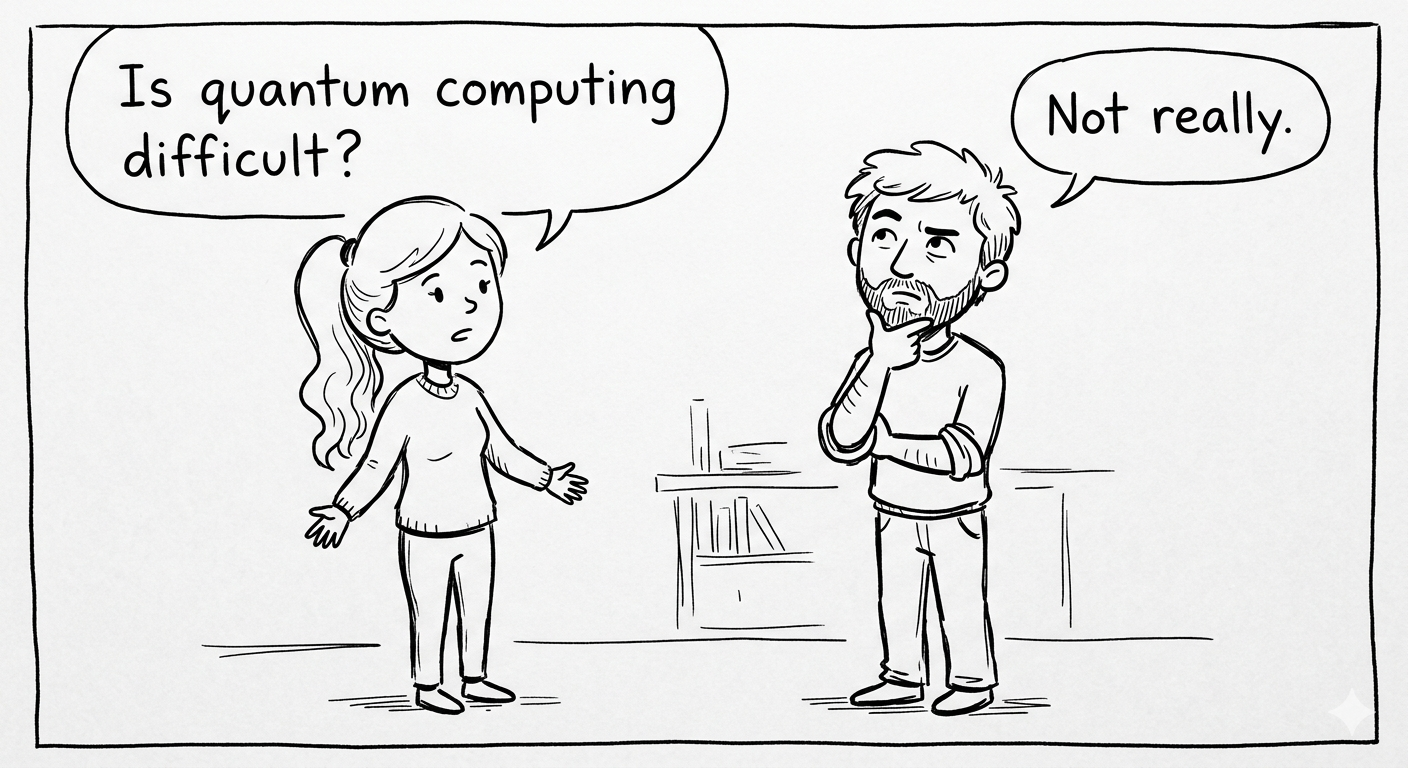
\includegraphics[width=0.8\textwidth]{figures/AliceandBob.png}
    \caption{Alice and Bob are discuss quantum computing. Image is generated by Gemini.}
    \label{fig: AliceandBob}
\end{figure}

In the world of quantum computing, there are really just two things you need to grasp: what it is and what it can do. That's it. Our journey will start with the simplest
symbols, then move on to basic quantum algorithms, simple quantum circuits, and finally
a small quantum computing project we'll build together. (Sounds exciting?)

Along the way, we'll also touch on some of the most important Python tools, such as PyTorch, TensorCircuit, TorchQuantum, and NumPy. If anything feels unclear, don't worry: you can always check the official documentation for more details.

To be honest, don't be scared by the name “quantum computing.” It's not as difficult as it sounds! You might be thinking: “But I don't have a background in quantum
mechanics or advanced mathematics.” Don't worry! All you really need is some basic linear algebra. If you do know a bit of quantum mechanics, that's fantastic, but it's by no means required. We'll keep things as simple as possible.

If you've read this far, it means you're curious about quantum computing, and that's the only thing you truly need. So thank you for joining! Now, Warriors, grab your armor and sword, your laptop and a piece of paper, and get ready to step into a whole new
world.

The references for this document are as follows:
\begin{referencebox}[Reference]
  \begin{itemize}
    \item \textit{Nielsen, M. A., \& Chuang, I. L. 2010. Quantum Computation and Quantum Information: 10th Anniversary Edition. Cambridge: Cambridge University Press.}
    \item \textit{Cohen-Tannoudji, C., Diu, B. and Laloe, F., 1986. Quantum mechanics, volume 1. Quantum Mechanics, John Wiley \& Sons.}
    \item \textit{Hajdušek, M. and Van Meter, R., 2023. Quantum communications. arXiv preprint arXiv:2311.02367.}
    \item \textit{姚 珩. 2018,「量子力學」, 滄海書局, 1-491頁。}
    \item \textit{TensorCircuit: \href{https://tensorcircuit.readthedocs.io/en/latest/}{https://tensorcircuit.readthedocs.io/en/latest/}}
    \item \textit{TorchQuantum: \href{https://hanruiwanghw.wixsite.com/torchquantum}{https://hanruiwanghw.wixsite.com/torchquantum}}
    \item \textit{PyTorch: \href{https://pytorch.org/}{https://pytorch.org/}}
  \end{itemize}
\end{referencebox}

Welcome to Quantum Computing. Let's make this journey fun!

\newpage
\section{The Cat, the Box, and the Collapse}
\label{basicinformation}
Quantum Computing is essentially the result of physicists and computer scientists going on a blind date and deciding to build a universe-sized calculator together. It's a field that hijacks the weirdest laws of quantum mechanics and forces them to cooperate with classical machine learning to create algorithms that are, \textit{theoretically}, at least, \textit{monstrously} powerful. 

But look, before we dive head-first into the deep end of the algorithmic pool, we need to clarify some basic information about Quantum Computing. Think of this as learning the rules of a game where the ball can be in two places at once and the referee is a complex number.

\subsection{Qubits and Quantum State}
In traditional computing, the basic unit of information is the bit, which is always either 0 or 1. We call this a Binary representation. In a classical sense, this means information is stored in discrete states. For example, in the frequency domain, a 1 can represent the presence of a signal while a 0 represents its absence. Similarly, in fields like machine learning, we use 1 for "True" and 0 for "False" in binary classification.

In quantum computing, the basic unit of information is the qubit. A qubit can exist in a state of 0, 1, or any superposition of these states. This means that, unlike a classical bit, a qubit can represent multiple states at the same time, allowing quantum algorithms to process a massive amount of information. The basic qubits are $\ket{0}$ and $\ket{1}$. The symbol $\ket{\cdot}$ is known as Dirac notation, which is used to represent a quantum state. In mathematics, we can convert Dirac notation into vectors, which are also called Ket states
\begin{equation}
    \ket{0} = \begin{bmatrix} 1 \\ 0 \end{bmatrix}, \quad \ket{1} = \begin{bmatrix} 0 \\ 1 \end{bmatrix}
\end{equation}

Since we have Ket states, we also have Bra states, denoted as $\bra{0}$ and $\bra{1}$
\begin{equation}
    \bra{0} = \begin{bmatrix} 1 & 0 \end{bmatrix}, \quad \bra{1} = \begin{bmatrix} 0 & 1 \end{bmatrix}
\end{equation}
The relationship between Bra and Ket states is defined by the inner product. For the basis states, we have $\braket{0|0} = 1$, $\braket{1|1} = 1$, and $\braket{0|1} = \braket{1|0} = 0$. This indicates that the basis states $\ket{0}$ and $\ket{1}$ are orthogonal to each other.In other words, a Bra state is the conjugate transpose of its corresponding Ket state. We represent this as $\bra{\psi} = \ket{\psi}^\dagger$, where the symbol $\dagger$ is pronounced as "dagger".

We can represent a general one-qubit state as a linear combination of these basis states
\begin{equation}
  \ket{\psi} = \alpha \ket{0} + \beta \ket{1}
  \label{eq: superposition}
\end{equation}
In this equation, $\alpha$ and $\beta$ are complex numbers that must satisfy the normalization condition: $|\alpha|^2 + |\beta|^2 = 1$.This condition ensures that the total probability remains 1. Specifically, the probabilities of measuring the qubit and finding it in state $\ket{0}$ or state $\ket{1}$ are given by $|\alpha|^2$ and $|\beta|^2$, respectively. This physical state of being in a combination of basis states is known as superposition.

\begin{SBUBox}{Superposition}
Superposition allows a system of $n$ qubits to represent $2^n$ states simultaneously.
\end{SBUBox}

We also have other common quantum states, such as $\ket{+}$ and $\ket{-}$, which are defined as
\begin{equation}
  \ket{+} = \frac{1}{\sqrt{2}} (\ket{0} + \ket{1}), \quad \ket{-} = \frac{1}{\sqrt{2}} (\ket{0} - \ket{1})
\end{equation}
Similarly, the states $\ket{i}$ and $\ket{-i}$ are defined as
\begin{equation}
  \ket{i} = \frac{1}{\sqrt{2}} (\ket{0} + i\ket{1}), \quad \ket{-i} = \frac{1}{\sqrt{2}} (\ket{0} - i\ket{1})
\end{equation}
For a single-qubit state, we can use the Bloch Sphere representation, as shown in Figure \ref{fig: bloch_sphere}. This is a geometrical way to visualize quantum states on the surface of a unit sphere.
\begin{figure}[h]
    \centering
    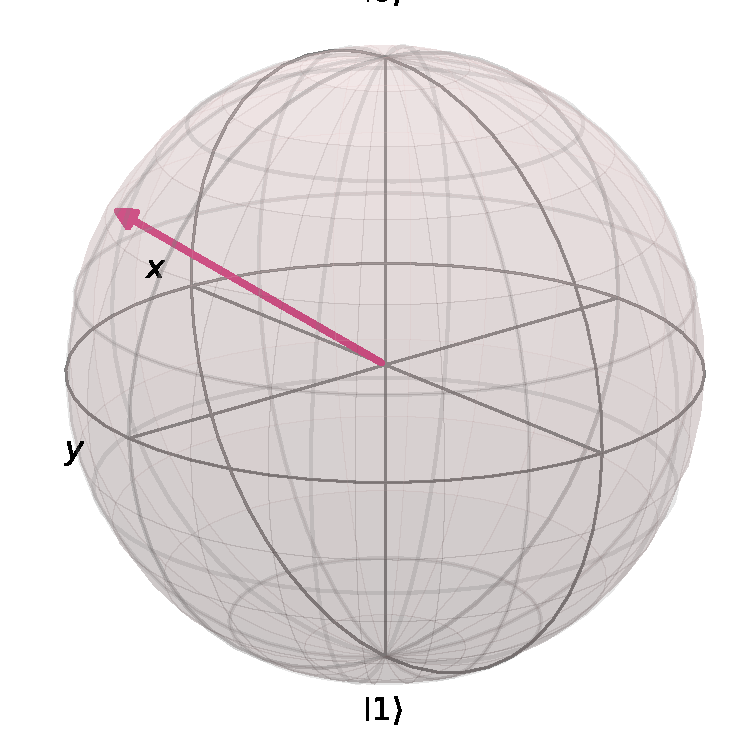
\includegraphics[width=0.3\textwidth]{figures/bloch_sphere.pdf}
    \caption{Bloch Sphere representation of a qubit state. The pink arrow represents a general quantum state vector $\ket{\psi}$ on the Bloch Sphere.}
    \label{fig: bloch_sphere}
\end{figure}

\begin{SBUBox}{Bloch Sphere}
The Bloch Sphere provides a visual tool for understanding qubits. The north and south poles represent the basis states $\ket{0}$ and $\ket{1}$, while states like $\ket{+}$ and $\ket{i}$ lie on the equator. Any point on the surface of the sphere corresponds to a pure quantum state.
\end{SBUBox}

As shown in Equation \ref{eq: superposition}, a general one-qubit state exists as a superposition of $\ket{0}$ and $\ket{1}$ simultaneously. Mathematically, a quantum state is a vector in Hilbert Space, which is a complex vector space. While a single qubit can represent two states at once, a system of $n$ qubits expands this capacity exponentially to $2^n$ simultaneous states.To construct high-dimensional quantum states, such as a two-qubit system, we use the tensor product ($\otimes$). A general two-qubit state can be expressed as:\begin{equation}\ket{\psi} = \alpha \ket{00} + \beta \ket{01} + \gamma \ket{10} + \delta \ket{11}\label{eq: two_qubit_state}\end{equation}The basis states of the combined system are created by taking the tensor product of the individual qubits' basis states. For example, the state $\ket{00}$ is the tensor product of two $\ket{0}$ states, resulting in a four-dimensional vector
\begin{equation}
  \ket{00} = \ket{0} \otimes \ket{0} = \begin{bmatrix} 1 \ 0 \end{bmatrix} \otimes \begin{bmatrix} 1 \ 0 \end{bmatrix} = \begin{bmatrix} 1 \ 0 \ 0 \ 0 \end{bmatrix}^T\label{eq: tensor_example}
\end{equation}
Similarly, the other basis states are constructed as follows
\begin{equation}
  \begin{aligned}
    \ket{01} = \ket{0} \otimes \ket{1} = \begin{bmatrix} 0 \ 1 \ 0 \ 0 \end{bmatrix}^T, \quad\ket{10} = \ket{1} \otimes \ket{0} = \begin{bmatrix} 0 \ 0 \ 1 \ 0 \end{bmatrix}^T, \quad\ket{11} = \ket{1} \otimes \ket{1} = \begin{bmatrix} 0 \ 0 \ 0 \ 1 \end{bmatrix}^T
  \end{aligned}
  \label{eq: tensor_product_all}
\end{equation}

\begin{SBUBox}{Scaling the State Space}
  The power of quantum computing lies in this exponential scaling. By using the tensor product, we can combine $n$ individual qubit Hilbert spaces into a single, massive $2^n$-dimensional space. This allows us to represent complex correlations, such as entanglement, which have no classical equivalent.
\end{SBUBox}

Using the tensor product, we can construct higher-dimensional quantum states from lower-dimensional ones. For example, a three-qubit state is created by taking the tensor product of a two-qubit state and a one-qubit state. This process can be repeated to represent multi-qubit systems of any dimension.

Quantum states are generally categorized into two types: \textbf{\textit{pure}} states and \textbf{\textit{mixed states}}. A pure state is described by a single ket vector in Hilbert space, such as the one in Equation \ref{eq: superposition}. In contrast, a mixed state represents a statistical mixture of different pure states and is described by a density matrix. Since a pure state can also be represented as a density matrix, this notation provides a universal way to describe any quantum system.The density matrix $\rho$ of a pure state is defined as
\begin{equation}
  \rho = \ket{\psi}\bra{\psi}
\end{equation}

More generally, a mixed state is represented by a sum of pure states weighted by their probabilities $p_i$
\begin{equation}
  \rho = \sum_i p_i \ket{\psi_i}\bra{\psi_i}
\end{equation}
where we use outer products to construct the matrix. 

To illustrate this, consider a quantum channel affected by bit-flip noise. This noise flips the input state with a certain probability. If the input is $\ket{\psi}$, the output of this channel can be represented as a mixed state
\begin{equation}
  \rho = p \ket{\psi}\bra{\psi} + (1-p) X \ket{\psi}\bra{\psi} X
\end{equation}

If we assume the input state is $\ket{\psi} = \ket{0}$, the Pauli-X gate will flip it to $\ket{1}$. The resulting output state becomes
\begin{equation}
  \rho = p \ket{0}\bra{0} + (1-p) \ket{1}\bra{1}
\end{equation}

The density matrix can be written explicitly in its matrix form
\begin{equation}
  \rho = \begin{bmatrix}p & 0 \\ 0 & 1-p\end{bmatrix}
  \label{eq: density_matrix}
\end{equation}

\begin{SBUBox}{Normalization and Trace}
  For a density matrix to be physically valid, it must be normalized. This is ensured by the trace, which is the sum of the diagonal elements of the matrix. For a general $2 \times 2$ matrix $A$
  \begin{equation*}
    A = \begin{bmatrix} a_{11} & a_{12} \\ a_{21} & a_{22} \end{bmatrix} \implies \text{Tr}(A) = a_{11} + a_{22}
  \end{equation*}
  For any density matrix $\rho$, the normalization condition requires that the trace equals one
  \begin{equation*}
    \text{Tr}(\rho) = 1
  \end{equation*}
\end{SBUBox}

So, for a general quantum state $\ket{\psi} = \alpha\ket{0}+\beta\ket{1}$, the density matrix is $\rho = \ket{\psi}\bra{\psi}$, the trace of this density matrix is
\begin{equation}
  \begin{aligned}
    \text{Tr}(\rho) &= \text{Tr}\begin{bmatrix}
      |\alpha|^2 & \alpha \beta^* \\
      \alpha^* \beta & |\beta|^2
    \end{bmatrix} \\
    & = |\alpha|^2 + |\beta|^2
  \end{aligned}
\end{equation}
and if we do the inner product of the same state
\begin{equation}
  \braket{\psi|\psi} = |\alpha|^2 + |\beta|^2
\end{equation}
we can get another very interesting conclusion: $\text{Tr}(\rho) = \braket{\psi|\psi} = 1$, this also proves the normalization. And we have another very interesting formula here 
\begin{equation}
  \text{Tr}(\ket{\psi}\bra{\psi}U) = \text{Tr}(U\ket{\psi}\bra{\psi}) = \bra{\psi}U\ket{\psi}
  \label{eq: tr_u}
\end{equation}

To manipulate and analyze quantum systems, we use several distinct types of multiplication rules. These operations allow us to combine, compare, and transform quantum states within the Hilbert space.
\begin{itemize}
  \item Tensor Product ($\otimes$): The tensor product is used to combine two or more quantum states into a larger, multi-qubit system. For example, if we have two qubits in states $\ket{\psi_1}$ and $\ket{\psi_2}$, their combined joint state is given by
  \begin{equation}
    \ket{\Psi} = \ket{\psi_1} \otimes \ket{\psi_2}
  \end{equation}
  \item Inner Product ($\braket{\cdot|\cdot}$): The inner product calculates the overlap between two quantum states, resulting in a complex scalar. For two states $\ket{\psi_1}$ and $\ket{\psi_2}$, the inner product is written as $\braket{\psi_1|\psi_2}$. This value represents the probability amplitude of transitioning from one state to another, where the actual probability is given by $|\braket{\psi_1|\psi_2}|^2$.
  \item Outer Product ($\ket{\cdot}\bra{\cdot}$): The outer product creates an operator or a matrix from two quantum states. For states $\ket{\psi_1}$ and $\ket{\psi_2}$, the outer product is defined as
  \begin{equation}
    O = \ket{\psi_1}\bra{\psi_2}
  \end{equation}
  Outer products are frequently used to construct \textbf{\textit{Projectors}}. A special case is the density matrix $\rho = \ket{\psi}\bra{\psi}$, which projects any state onto the vector $\ket{\psi}$.
\end{itemize}

\begin{SBUBox}{Memorize the Operations}
A simple way to remember these is by their resulting dimensions. The Inner Product ($1 \times 2$ matrix times $2 \times 1$) results in a scalar. The Outer Product ($2 \times 1$ matrix times $1 \times 2$) results in a $2 \times 2$ matrix. The Tensor Product combines the dimensions, for example, turning two 2-dimensional vectors into one 4-dimensional vector.
\end{SBUBox}


\subsection{Quantum Operations and Quantum Operators}
In this section, we will discuss basic quantum operations and quantum gates. Quantum gates serve as the fundamental building blocks of quantum circuits and are used to manipulate quantum states. These gates are represented by unitary matrices, which possess the unique property of preserving the inner product of quantum states. This ensures that the total probability of all possible measurement outcomes remains equal to one throughout the computation.

A matrix $U$ is considered unitary if it satisfies the condition
\begin{equation}
  U^\dagger U = U U^\dagger = I
\end{equation}
where $I$ is the identity matrix and $U^\dagger$ is the conjugate transpose of $U$. Because quantum gates must be unitary, every quantum operation is inherently reversible, meaning we can always "undo" a gate by applying its adjoint.

\begin{SBUBox}{Unitary Evolution}
  If we apply a unitary operator $U$ to a normalized state $\ket{\psi}$, the state remains normalized after the transformation. This can be shown mathematically as follows
  \begin{equation*}
    \langle \psi | U^\dagger U | \psi \rangle = \braket{\psi|\psi} = 1
  \end{equation*}
\end{SBUBox}

Quantum gates (quantum operators) are represented by unitary matrices that act on the state vectors. Below are the most frequently used gates in quantum circuit design and quantum transformation.
\begin{itemize}
  \item \textbf{Pauli-X Gate}: Also known as the NOT gate or a bit-flip gate, the Pauli-X gate maps $\ket{0}$ to $\ket{1}$ and vice versa. Its matrix representation is
  \begin{equation}
    X = \begin{bmatrix} 0 & 1 \\ 1 & 0 \end{bmatrix}
  \end{equation}
  \item \textbf{Pauli-Y Gate}: The Pauli-Y gate performs a complex rotation that combines both a bit-flip and a phase-flip. It is defined by the matrix
  \begin{equation}
    Y = \begin{bmatrix} 0 & -i \\ i & 0 \end{bmatrix}
  \end{equation}
  \item \textbf{Pauli-Z Gate}: The Pauli-Z gate applies a phase flip to the $\ket{1}$ state (change it to $-\ket{1}$) while leaving the $\ket{0}$ state unchanged. Its matrix representation is
  \begin{equation}
    Z = \begin{bmatrix} 1 & 0 \\ 0 & -1 \end{bmatrix}
  \end{equation}
  \item \textbf{Hadamard Gate}: The Hadamard gate ($H$) is fundamental for generating superposition. It transforms the computational basis states $\{\ket{0}, \ket{1}\}$ into the diagonal basis states $\{\ket{+}, \ket{-}\}$ respectively
  \begin{equation}
    H = \frac{1}{\sqrt{2}} \begin{bmatrix} 1 & 1 \\ 1 & -1 \end{bmatrix}
  \end{equation}
  \item \textbf{Control Not Gate}: The CNOT gate is a critical two-qubit gate used to create entanglement. It flips the state of the target qubit (the second qubit) if and only if the control qubit (the first qubit) is in the state $\ket{1}$
  \begin{equation}
    \text{CNOT} = \begin{bmatrix} 1 & 0 & 0 & 0 \\ 0 & 1 & 0 & 0 \\ 0 & 0 & 0 & 1 \\ 0 & 0 & 1 & 0 \end{bmatrix}
  \end{equation}
\end{itemize}

\begin{SBUBox}{Unitary and Self-Adjoint}
Notice that the Pauli gates and the Hadamard gate are not only unitary but also Hermitian ($A = A^\dagger$). This implies that they are their own inverses. Applying the same gate twice, such as $H^2$ or $X^2$, will return the qubit to its original state, equivalent to the Identity operation $I$.
\end{SBUBox}

These gates can be combined to create complex quantum circuits, enabling a wide range of quantum algorithms and protocols. To understand their operation, we can examine the specific action of the Pauli-Z gate on the basis states

\begin{equation}
  \begin{aligned}
  Z \ket{0} &= \begin{bmatrix} 1 & 0 \\ 0 & -1 \end{bmatrix} \begin{bmatrix} 1 \\ 0 \end{bmatrix} = \begin{bmatrix} 1 \\ 0 \end{bmatrix} = \ket{0} \\
  Z \ket{1} &= \begin{bmatrix} 1 & 0 \\ 0 & -1 \end{bmatrix} \begin{bmatrix} 0 \\ 1 \end{bmatrix} = \begin{bmatrix} 0 \\ -1 \end{bmatrix} = -\ket{1}
  \end{aligned}
\end{equation}

As we talked about above, a quantum gate operates on the left side of a Ket state. In this context, all quantum gates are considered operators. If an operator satisfies the condition $U U^\dagger = U^\dagger U = I$, it is defined as a Unitary operator. This property ensures that every quantum gate has an inverse, which is its adjoint (conjugate transpose). When applying an operation to a Bra state, the operator acts from the right as its adjoint, written as $\bra{\psi} U^\dagger$.

\begin{SBUBox}{The Adjoint Operation}
The relationship between the action on Kets and Bras follows the dual vector space rules. If the evolution of a Ket is $U\ket{\psi}$, the corresponding evolution of the Bra is
\begin{equation*}
  (U\ket{\psi})^\dagger = \bra{\psi}U^\dagger
\end{equation*}
\end{SBUBox}

The Pauli gates and the Hadamard gate discussed previously are single-qubit gates, meaning they operate on an individual qubit. In contrast, the CNOT gate is a two-qubit gate that acts on a pair of qubits simultaneously. Beyond these, we can also utilize more complex multi-qubit gates, such as the Toffoli gate (CCNOT) or the Fredkin gate (Controlled-SWAP).

A common method to construct multi-qubit gates is by taking the tensor product of single-qubit gates. For example, if we wish to apply a Hadamard gate to the first qubit and a Pauli-X gate to the second qubit, the resulting two-qubit operator is given by the tensor product

\begin{equation}
  H \otimes X = \frac{1}{\sqrt{2}} \begin{bmatrix} 1 & 1 \\ 1 & -1 \end{bmatrix} \otimes \begin{bmatrix} 0 & 1 \\ 1 & 0 \end{bmatrix} = \frac{1}{\sqrt{2}} \begin{bmatrix} 0 & 1 & 0 & 1 \\ 1 & 0 & 1 & 0 \\ 0 & 1 & 0 & -1 \\ 1 & 0 & -1 & 0 \end{bmatrix}
\end{equation}

\begin{SBUBox}{Independent Operations}
When we represent a gate as $A \otimes B$, it mathematically signifies that the operations $A$ and $B$ are being performed independently and simultaneously on their respective qubits. The dimension of the resulting matrix always scales as $2^n \times 2^n$. For a two-qubit system, this results in a $4 \times 4$ matrix
\begin{equation*}
  (A \otimes B) (\ket{\psi_1} \otimes \ket{\psi_2}) = (A\ket{\psi_1}) \otimes (B\ket{\psi_2})
\end{equation*}
\end{SBUBox}

\subsection{Measurement and Fidelity}
In quantum mechanics, the famous Schrödinger's cat (Figure \ref{fig: schrodinger'scat}) thought experiment illustrates the counterintuitive concepts of superposition and measurement. In this scenario, a cat is placed in a sealed box with a radioactive atom that has a 50\% chance of decaying within an hour. If the atom decays, it triggers a mechanism that releases a poison, killing the cat; if not, the cat remains alive.
\begin{figure}[h]
    \centering
    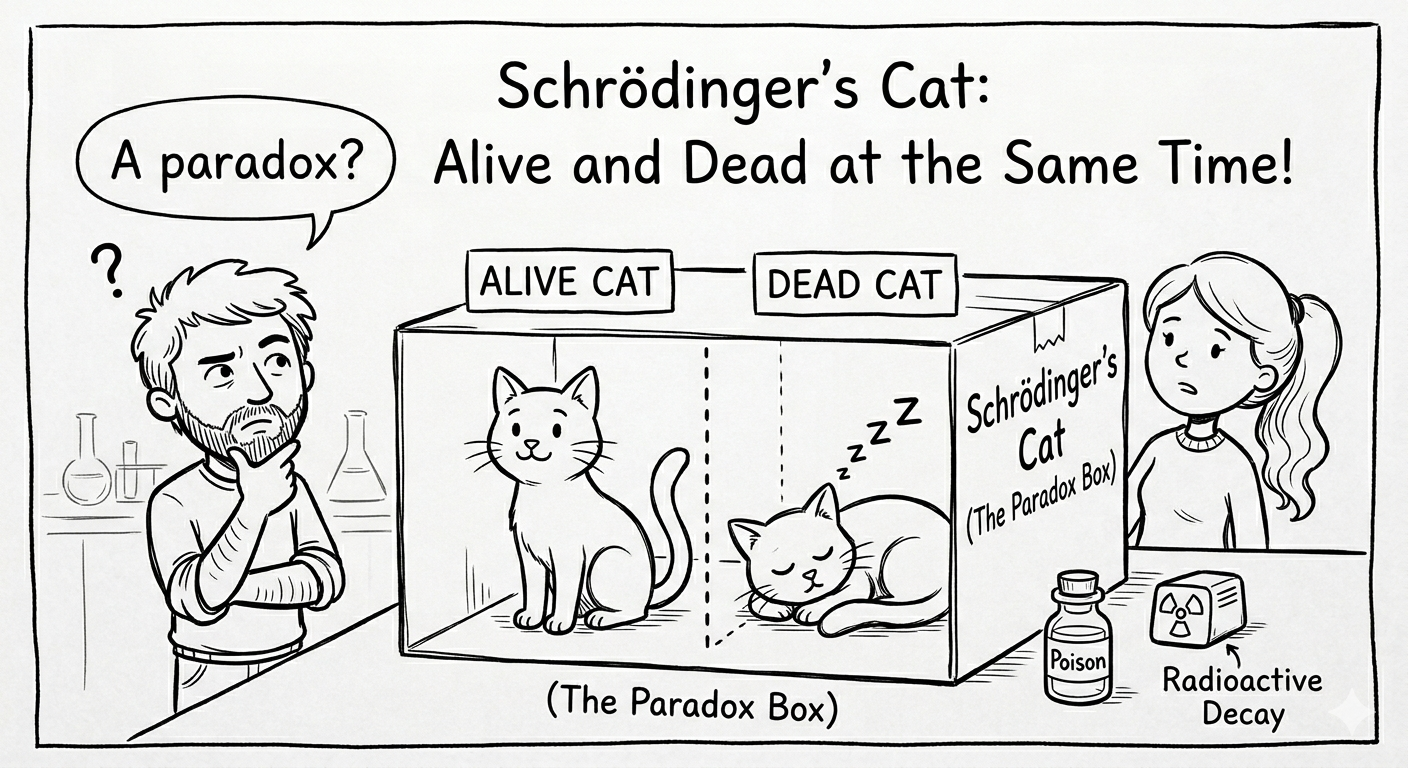
\includegraphics[width=0.8\textwidth]{figures/schrodinger_scat.png}
    \caption{Alice and Bob are discuss Schrödinger's cat. Image is generated by Gemini.}
    \label{fig: schrodinger'scat}
\end{figure}

According to the principles of quantum mechanics, until the box is opened and the system is observed, the cat exists in a superposition of being both alive and dead simultaneously. This joint state can be represented as
\begin{equation}
\ket{\psi} = \frac{1}{\sqrt{2}} (\ket{\text{Alive}} + \ket{\text{Dead}})
\end{equation}

The act of "opening the box" constitutes a measurement. It is only after this observation that we can say the cat is either alive or dead. Once the measurement occurs, the superposition collapses into one of the possible basis states. This illustrates a fundamental principle: the act of measurement fundamentally alters the state of the system. The resulting state is known as the post-measurement state.

\begin{SBUBox}{Copenhagen Interpretation}
The Copenhagen interpretation of Quantum Physics was developed by Niels Bohr and his assistant, Werner Heisenberg, between 1925 and 1927. It is based on the proposition that Physics is the Science of measurement and that a measurable quantity has no reality until it is measured. In the Copenhagen interpretation, one applies the rules of Quantum Mechanics to sub-microscopic systems but not to the measuring device, which is a macroscopic object that has the property (for reasons which are not understood) of effecting wavefunction collapse from a quantum superposition to a classical probabilistic state. Moreover, the act of "observing" or "measuring" an object is irreversible, and no truth can be attributed to an object except according to the results of its measurement (that is, the Copenhagen interpretation rejects counterfactual definiteness)
\end{SBUBox}

To perform a measurement, we must first define the basis states of the system, which serve as the fundamental units of the entire quantum state space. The measurement process involves projecting the quantum state onto one of these basis states, with each state corresponding to a specific physical outcome. As discussed previously, the most common basis consists of $\ket{0}$ and $\ket{1}$, which are the eigenstates of the Pauli-Z operator and are thus referred to as the \textbf{\textit{Z-basis}}.

However, the computational \textbf{\textit{Z-basis}} is not the only way to observe a qubit. We also frequently use the \textbf{\textit{X-basis}} and \textbf{\textit{Y-basis}}, which represent measurements along different axes of the Bloch sphere. These bases are defined as follows
\begin{equation}
  \begin{aligned}
    \ket{+} = \frac{1}{\sqrt{2}}(\ket{0} + \ket{1}), \quad & \ket{-} = \frac{1}{\sqrt{2}}(\ket{0} - \ket{1}) \\
    \ket{+i} = \frac{1}{\sqrt{2}}(\ket{0} + i\ket{1}), \quad & \ket{-i} = \frac{1}{\sqrt{2}}(\ket{0} - i\ket{1})
  \end{aligned}
\label{eq: x_y_basis}
\end{equation}

\begin{SBUBox}{Changing Bases}
In a quantum circuit, we usually only have hardware that measures in the Z basis. For example, to measure in the X basis, we apply a Hadamard gate ($H$) before the measurement to rotate the X basis states into the Z basis. All the things we need to do is transform the measurement basis through some unitary operators. This is mathematically equivalent to a change of basis transformation
\begin{equation*}
\ket{\psi} \xrightarrow{U} \ket{\psi'} \xrightarrow{\text{Measure } Z} \text{Outcome}
\end{equation*}
This technique allows us to extract information from any direction on the Bloch sphere using only a standard Z-measurement (or any other measurement).
\end{SBUBox}

You may find something real interesting: the X basis and Y basis are fundamentally superpositions of the Z basis. Consequently, choosing a different measurement basis will lead to different physical outcomes and probabilities.

For a qubit in a general state $\ket{\psi} = \alpha \ket{0} + \beta \ket{1}$, a measurement in the Z basis yields $\ket{0}$ with probability $|\alpha|^2$ and $\ket{1}$ with probability $|\beta|^2$. If we choose to measure in the X basis, the outcomes are $\ket{+}$ with probability $|\frac{\alpha + \beta}{\sqrt{2}}|^2$ and $\ket{-}$ with probability $|\frac{\alpha - \beta}{\sqrt{2}}|^2$. Similarly, measuring in the Y basis results in $\ket{+i}$ with probability $|\frac{\alpha + i\beta}{\sqrt{2}}|^2$ and $\ket{-i}$ with probability $|\frac{\alpha - i\beta}{\sqrt{2}}|^2$.

The measurement process consists of two primary steps: first, identifying the basis states of the chosen observable, and second, projecting the quantum state onto those basis states. We can calculate the probabilities for the Z-basis measurement as follows

\begin{equation}
  \begin{aligned}
    \text{Prob}\{1\} & = |\braket{0|\psi}|^2 \\
    & = |\bra{0}(\alpha \ket{0} + \beta \ket{1})|^2 \\
    & = |\alpha \braket{0|0} + \beta \braket{0|1}|^2 \\
    & = |\alpha \times (1) + \beta \times (0)|^2 \\
    & = |\alpha|^2 \\
    \text{Prob}\{-1\} & = |\braket{1|\psi}|^2 \\
    & = |\bra{1}(\alpha \ket{0} + \beta \ket{1})|^2 \\
    & = |\alpha \braket{1|0} + \beta \braket{1|1}|^2 \\
    & = |\alpha \times (0) + \beta \times (1)|^2 \\
    & = |\beta|^2
  \end{aligned}
\label{eq: z_basis_measurement}
\end{equation}

The zeros in Equation \ref{eq: z_basis_measurement} appear because the basis states $\ket{0}$ and $\ket{1}$ are orthogonal, meaning their inner product is zero: $\braket{0|1} = 0$. Conversely, since the basis is normalized, the inner product with themselves is unity: $\braket{0|0} = 1$ and $\braket{1|1} = 1$. This link between the state vector amplitudes and the observed probabilities is a fundamental principle known as the \textbf{\textit{Born rule}}.

\begin{SBUBox}{The Born Rule}
The Born Rule states that for a quantum system in state $\ket{\psi}$, the probability of obtaining a specific outcome corresponding to the eigenvector $\ket{n}$ is given by the square of the magnitude of the probability amplitude
\begin{equation*}
P(n) = |\braket{n|\psi}|^2
\end{equation*}
This rule bridges the gap between the abstract complex vector space of quantum mechanics and the real-world statistical results of experiments.
\end{SBUBox}

Here we face a problem, ok, now I have probability, what about the expectation and variance? After determining the probabilities of individual outcomes, we can calculate the expectation value, which represents the average result of a measurement performed many times on identically prepared quantum states. In probability theory, the expectation is defined as the sum of each possible outcome multiplied by its corresponding probability.

In our example, we denote the observable as $Z$ because the measurement is performed in the $Z$ basis. The possible outcomes (eigenvalues) of the Pauli-Z operator are $+1$ (corresponding to $\ket{0}$) and $-1$ (corresponding to $\ket{1}$). Therefore, the expectation value $\mathbb{E}[Z]$, often written as $\braket{Z}$ in physics notation, is given by the sum of these products
\begin{equation}
  \begin{aligned}
    \mathbb{E}[Z] &= \text{Prob}\{+1\} \cdot (+1) + \text{Prob}\{-1\} \cdot (-1) \\
    &= |\alpha|^2 - |\beta|^2
  \end{aligned}
\label{eq: expectation_value}
\end{equation}

This is in linear algebra way, but, we can also express the expectation value using the dirac notation
\begin{equation}
    \braket{Z} = \bra{\psi} Z \ket{\psi} 
\end{equation}
if you really don't like the dirac notation, well, we still can use matrix to represent the operators and states. In matrix form, the expectation value can be computed as
\begin{equation}
  \begin{aligned}
    \braket{Z} &= \begin{pmatrix} \alpha^* & \beta^* \end{pmatrix} \begin{pmatrix} 1 & 0 \\ 0 & -1 \end{pmatrix} \begin{pmatrix} \alpha \\ \beta \end{pmatrix} \\
    &= \begin{pmatrix} \alpha^* & \beta^* \end{pmatrix} \begin{pmatrix} \alpha \\ -\beta \end{pmatrix} \\
    &= |\alpha|^2 - |\beta|^2
  \end{aligned}
\end{equation}

Once the expectation value is determined, then we want to know the variance. In probability and statistics, variance is defined as the expectation of the squared deviation from the mean. For our observable $Z$, the variance is given by the difference between the expectation of the square and the square of the expectation
\begin{equation}
  \begin{aligned}
    \text{Var}(Z) &= \mathbb{E}[Z^2] - (\mathbb{E}[Z])^2 \\
    &= \text{Prob}\{+1\} \cdot (+1)^2 + \text{Prob}\{-1\} \cdot (-1)^2 - \left( |\alpha|^2 - |\beta|^2 \right)^2 \\
    &= |\alpha|^2 + |\beta|^2 - \left( |\alpha|^2 - |\beta|^2 \right)^2 \\
    &= 1 - \left( |\alpha|^2 - |\beta|^2 \right)^2
  \end{aligned}
\end{equation}

Do you still remember the \textit{Outer Product}? We can have a new operator by doing outer product, right? Technically, this is called \textbf{\textit{Projector}}. We can also use projector to calculate the probability of a measurement outcome. For example, the probability of measuring $\ket{0}$ can be calculated using the projector $\ket{0}\bra{0}$ as follows
\begin{equation}
  \begin{aligned}
    \text{Prob}\{+1\}  &= \bra{\psi} \ket{0}\bra{0} \ket{\psi} \\
    &= \braket{\psi | 0} \cdot \braket{0 | \psi} \\
    &= \braket{0|\psi} \cdot \braket{\psi|0} \\
    &= |\braket{0|\psi}|^2
  \end{aligned}
  \label{eq: project_measure}
\end{equation}
in the matrix form
\begin{equation}
  \begin{aligned}
    \text{Prob}\{+1\}  &= \begin{pmatrix} \alpha^* & \beta^* \end{pmatrix} \begin{pmatrix} 1 & 0 \\ 0 & 0 \end{pmatrix} \begin{pmatrix} \alpha \\ \beta \end{pmatrix} \\
    &= \begin{pmatrix} \alpha^* & \beta^* \end{pmatrix} \begin{pmatrix} \alpha \\ 0 \end{pmatrix} \\
    &= |\alpha|^2
  \end{aligned}
\end{equation}

Equation \ref{eq: project_measure} is indeed very familiar. If we replace the specific computational basis projector $\ket{0}\bra{0}$ with a general projector $U = \ket{\phi}\bra{\phi}$, the probability of the system $\ket{\psi}$ collapsing onto $\ket{\phi}$ is given by the inner product $\bra{\psi} U \ket{\psi}$. This structure is identical to the expectation value formula we saw in Equation \ref{eq: tr_u}. This "Trace Rule" is incredibly powerful because it works for both pure states and mixed states.

Once we understand how to perform measurements, we often need a metric to quantify the similarity between two quantum states. This is provided by \textbf{\textit{Fidelity}}, which serves as a measure of how "close" two quantum states are to each other in Hilbert space.

For two pure states, $\ket{\psi}$ and $\ket{\phi}$, the fidelity is defined as the squared overlap between them
\begin{equation}
  F(\psi, \phi) = |\braket{\psi|\phi}|^2
\end{equation}

In experimental settings, we often deal with mixed states due to noise or decoherence. A mixed state is represented by a density matrix $\rho$. In the common case where we want to compare an experimental mixed state $\rho$ with an ideal pure target state $\ket{\psi}$, the fidelity is defined as
\begin{equation}
  F(\rho, \ket{\psi}) = \bra{\psi}\rho\ket{\psi}
\end{equation}

Here, $\rho$ represents the actual state prepared in the laboratory, while $\ket{\psi}$ is the theoretical state we aimed to achieve. The fidelity value $F$ always ranges from 0 to 1
\begin{equation*}
  0 \le F \le 1
\end{equation*}

A fidelity of 1 indicates that the two states are identical, while a fidelity of 0 indicates that the states are perfectly orthogonal. In quantum computing benchmarks, a "high-fidelity" gate or state (e.g., $F > 0.99$) is essential for fault-tolerant computation.

\begin{SBUBox}{Expressibility via KL Divergence}
The Expressibility ($Expr$) of a quantum circuit is defined as the KL Divergence of its sampled fidelity distribution $P_{pqc}(F)$ from the Haar random distribution $P_{Haar}(F)$
\begin{equation*}
Expr = D_{KL} \left( P_{pqc}(F) | P_{Haar}(F) \right)
\end{equation*}
For a Hilbert space of dimension $N = 2^n$, the probability density function for the fidelity $F$ of Haar-random states is given by
\begin{equation*}
P_{Haar}(F) = (N - 1)(1 - F)^{N - 2}
\end{equation*}
In this context, $F = |\braket{\psi(\theta_1) | \psi(\theta_2)}|^2$ is treated as a random variable obtained by sampling pairs of parameters $(\theta_1, \theta_2)$. A lower $Expr$ value (closer to 0) indicates a highly expressible circuit that can uniformly explore the state space.
\end{SBUBox}

\subsection{Entanglement}
Well, people always ask: what is entanglement? This seems to be the most difficult question in the quantum realm. Indeed, grasping the true nature of entanglement is no simple feat, as it defies our classical intuition of local reality. To get our feet wet, let's start with a common (and technically incorrect) daily example to set the stage.

Imagine Alice has a pair of gloves. Alice places each glove in a separate box and send one to a Bob in New York and the Eve in London. The moment your friend in London opens the box and finds a Left-hand glove, they instantly know that the glove in London must be the Right-hand one, shown in Figure \ref{fig: entanglegloves}.
\begin{figure}[h]
    \centering
    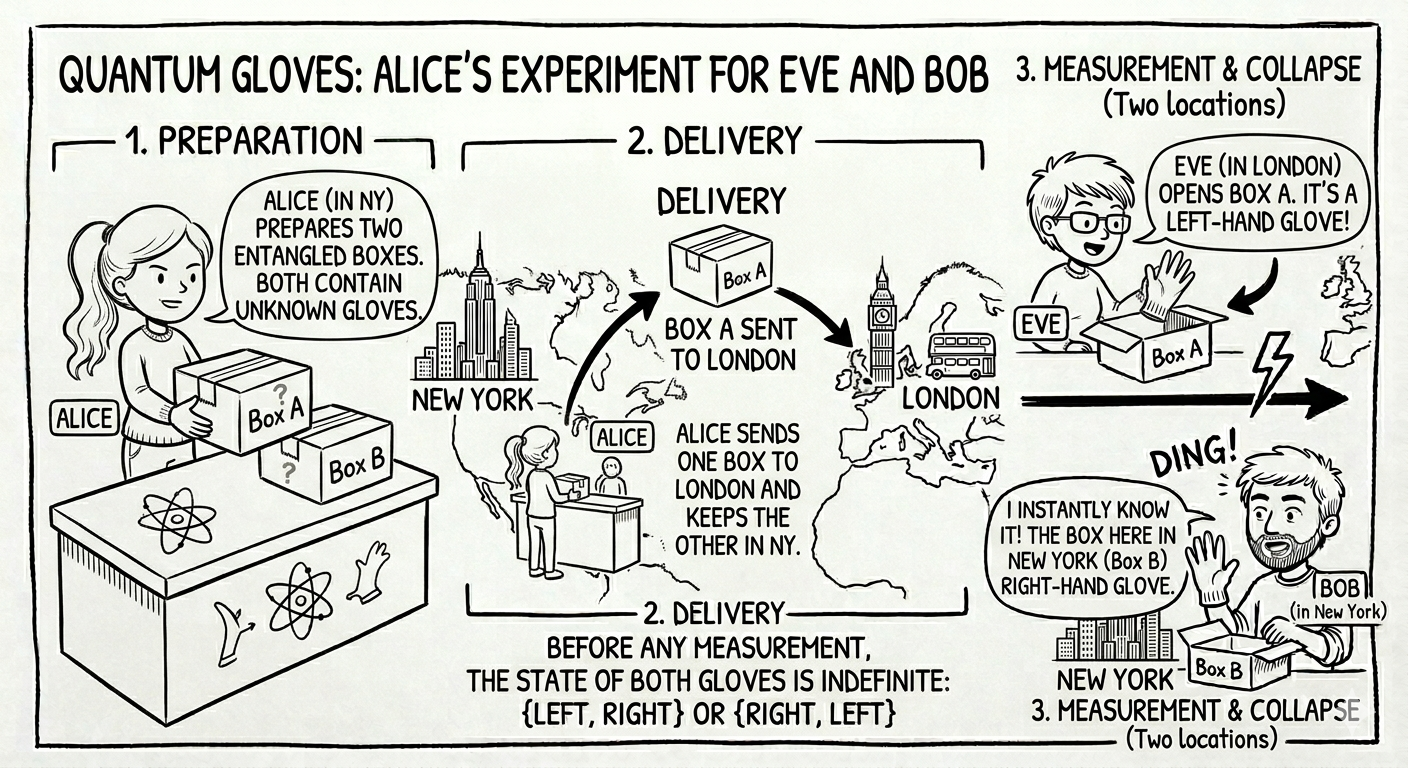
\includegraphics[width=0.8\textwidth]{figures/entanglegloves.png}
    \caption{Alice, Bob and Eve are doing gloves experiment. Image is generated by Gemini.}
    \label{fig: entanglegloves}
\end{figure}

In this classical case, the "state" of the gloves was determined the moment you packed them. However, in the quantum world, the gloves are neither left nor right until someone looks. They exist in a superposition, and the "choice" made by one particle instantly dictates the state of its partner, regardless of the distance between them.

To move from "gloves" to the rigorous world of Hilbert space, we must first distinguish between the \textbf{\textit{Global State}} of a collective system and the \textbf{\textit{Local States}} of its individual constituents.

In classical mechanics, describing a global system is as simple as listing the properties of its local parts. In the quantum system, however, the global state can contain information that is completely absent from its local components.

A Global State refers to the entire quantum system, often denoted as a composite state vector $\ket{\psi}_{AB}$ or a density matrix $\rho_{AB}$ living in a joint Hilbert space $\mathcal{H}_A \otimes \mathcal{H}_B$. Conversely, a Local State refers to the state of a specific subsystem (e.g., just qubit $A$ or just qubit $B$)

Let's look at a very easy example, we have a global state $\ket{\psi} = \ket{\rho} \otimes \ket{\phi} $, what are the local states? Bravo! They are $\ket{\rho}$ and $\ket{\phi}$. As you can see here, the pure global state $\ket{\psi}$ can be written as the tensor product of two local states, we also call this global state the \textbf{\textit{Product State}}.

Alright, let's do some math, if we have a state $\ket{\psi} = \frac{1}{2}(\ket{00}+\ket{01}+\ket{10}+\ket{11})$, we can immediately know the local states
\begin{equation}
  \begin{aligned}
    \ket{\psi} &= \frac{1}{2}(\ket{00}+\ket{01}+\ket{10}+\ket{11}) \\
    & = \frac{1}{\sqrt{2}}(\ket{0}+\ket{1}) \otimes \frac{1}{\sqrt{2}}(\ket{0}+\ket{1}) \\
    & = \ket{\rho} \otimes \ket{\phi}
  \end{aligned}
  \label{eq: product_state}
\end{equation}

In such a case, the local states are well-defined as the tensor product of the pure states $\ket{\rho}$ and $\ket{\phi}$. However, when a state is Entangled, the global state \textbf{\textit{cannot}} be factored.

\begin{SBUBox}{Proof: Entanglement}
Consider the most famous global state, the Bell state $\ket{\Phi^+}$
\begin{equation*}
  \ket{\Phi^+} = \frac{1}{\sqrt{2}}(\ket{00} + \ket{11})
\end{equation*}
If we attempt to find local states $\ket{\psi}_A = a\ket{0} + b\ket{1}$ and $\ket{\psi}_B = c\ket{0} + d\ket{1}$ such that their product equals $\ket{\Phi^+}$, we yield
\begin{equation*}
  (a\ket{0} + b\ket{1}) \otimes (c\ket{0} + d\ket{1}) = ac\ket{00} + ad\ket{01} + bc\ket{10} + bd\ket{11}
\end{equation*}
Matching this to our Bell state requires the "cross-terms" $\ket{01}$ and $\ket{10}$ to vanish, meaning $ad = 0$ and $bc = 0$. But if $a=0$ or $d=0$, the coefficients for $\ket{00}$ or $\ket{11}$ would also vanish. This contradiction proves that the global state $\ket{\Phi^+}$ contains "correlations" that cannot be assigned to any local state.
\end{SBUBox}

\newpage
\section{Quantum Die: Rolling the Famous States}
Congratulation, you have finished the section \ref{basicinformation}! Not too hard, right? After understand some basic knowledge of quantum computing, now in this section, we will discuss some famous quantum states that can be used in many aspects.
\begin{figure}[h]
    \centering
    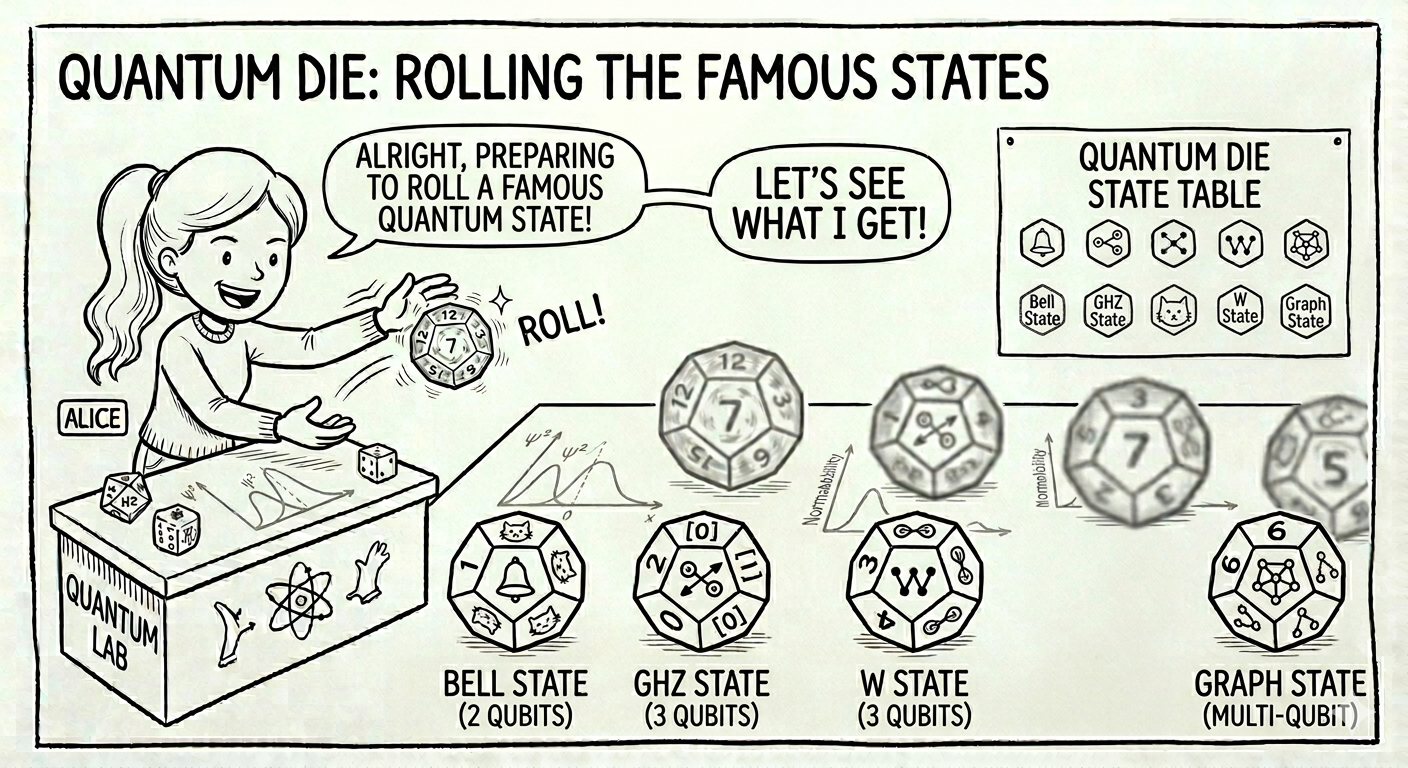
\includegraphics[width=0.8\textwidth]{figures/quantumrolling.png}
    \caption{Alice is doing quantum rolling experiment, she has the probability to get four different quantum states. Image is generated by Gemini.}
    \label{fig: quantumrolling}
\end{figure}

\subsection{Bell States}
Well, we actually meet bell states before, you still remember when we trying to figure out the difference between product state and entangled state? We use the bell state to be our example. So, what bell states exactly are?

Bell states, or, Einstein-Podolsky-Rosen (EPR) pairs, are very special two-qubit quantum state in two-qubit system, there represent the simplest example of quantum entangled states or quantum entanglement. We have four different bell states
\begin{equation}
  \begin{aligned}
    \ket{\Phi^+} &= \frac{1}{\sqrt{2}}(\ket{00} + \ket{11}) \\
    \ket{\Phi^-} &= \frac{1}{\sqrt{2}}(\ket{00} - \ket{11}) \\
    \ket{\Psi^+} &= \frac{1}{\sqrt{2}}(\ket{01} + \ket{10}) \\
    \ket{\Psi^-} &= \frac{1}{\sqrt{2}}(\ket{01} - \ket{10}) \\
  \end{aligned}
\end{equation}

Bell states also can be used as basis, for example, for a general two-qubit quantum state $\ket{\psi} = a_0\ket{00} + a_1\ket{01}+a_2\ket{10}+a_3\ket{11}$, the probability amplitude should satisfies the normalization which means $|a_0|^2+|a_1|^2+|a_2|^2+|a_3|^2 = 1$, and we can rewrite this quantum state under bell basis
\begin{equation}
  \ket{\psi} = \frac{a_0+a_3}{\sqrt{2}}\ket{\Phi^+} + \frac{a_0-a_3}{\sqrt{2}}\ket{\Phi^-} + \frac{a_1+a_2}{\sqrt{2}}\ket{\Psi^+} + \frac{a_1-a_2}{\sqrt{2}}\ket{\Psi^-}
\end{equation}

I bet you definitely want to know how to measure bell states, as so far we only talk about one-qubit measurement. In fact, it's the same, we use the projector. Same steps, first, define which basis, second, create the projector, third, get the outcomes; but here, slightly difference, we need to understand which qubit we want to measure since we have two qubits right now, we named the first A and second qubit B (always for Alice and Bob!). Let's do the measurement under Z basis, this is always the easiest example.
\begin{itemize}
  \item Measure on the first qubit: If we only want to measure the first qubit, the projector for the first qubit should be $\ket{0}_A\bra{0}$, and the same time, we do nothing to the second qubit, so there shoud be one identical operator $I$ for the second qubit. In all, the projector is written as $\Pi_{Z, +}^{A} = \ket{0}_A\bra{0} \otimes I$. Here, $\Pi_{Z, +}^{A}$ represents the projector that doing Z plus ($\ket{0}$) measurement on the first qubit.
  \item Measure on the second qubit: I think you can write the projector down right now since this process is exactly the same as measure on the first qubit.
  \item Measure on both qubits: We also use the projector, but this time, the projector should be like $\Pi_{Z, +}^{A, B} = \ket{0}_A\bra{0} \otimes \ket{0}_B\bra{0}$.
\end{itemize}

Now we know the projectors we need to measure the bell states. But how the projector works (hint: don't forget the trace rule)? Let's see the measurement on the first qubit for the $\ket{\Phi^+}$ state.
\begin{equation}
  \begin{aligned}
    \text{Prob\{+1\}}_A &= \text{Tr}(\Pi_{Z, +}^{A}\ket{\Phi^+}_A\bra{\Phi^+}) \\
    &= \bra{\Phi^+}_A \Pi_{Z, +}^{A} \ket{\Phi^+} \\
    & = \frac{1}{\sqrt{2}}(\bra{00} + \bra{11})(\ket{0}_A\bra{0} \otimes I)\frac{1}{\sqrt{2}}(\ket{00} + \ket{11}) \\
    & = \frac{1}{2}(\bra{00}\ket{0}_A\bra{0} \otimes I\ket{00})(\bra{00}\ket{0}_A\bra{0} \otimes I\ket{11})(\bra{11}\ket{0}_A\bra{0} \otimes I\ket{00})(\bra{11}\ket{0}_A\bra{0} \otimes I\ket{11}) \\
    & = \frac{1}{2}
  \end{aligned}
\end{equation}
You may ask, how we compute this part $\bra{00}\ket{0}_A\bra{0} \otimes I\ket{00}$? The process as follows
\begin{equation}
  \begin{aligned}
    \bra{00}_{AB}(\ket{0}_A\bra{0} \otimes I)\ket{00}_{AB} &= \bra{0}_A(\ket{0}_A\bra{0})\ket{0}_A\bra{0}_BI\ket{0}\\
    & =  (\braket{0|0}_A)(\braket{0|0}_A)(\braket{0|0}_B) \\
    & = 1
  \end{aligned}
\end{equation}
other parts also compute like this.

Imagine that Alice and Bob share one $\ket{\Phi}^+$ state, for the whole system, the trace of the density matrix is $\text{Tr}(\rho) = \text{Tr}(\ket{\Phi}^+\bra{\Phi}^+) = 1$ which means the system contains whole information, there is a perfectly entanglement between Alice and Bob. Now, is time for Bob to explore the universe, so Bob take his qubit B to the Mars, and Alice now only has her qubit A. If Alice doesn't want to care about what happens to Bob, so Alice need to do \textbf{\textit{Partial Trace}} of the entangled $\ket{\Phi}^+$ state. 
\begin{SBUBox}{Partial Trace}
  The definition of the partial trace is remarkably straightforward: to remove system $B$, we perform the trace operation only on the $B$ component while leaving system $A$ untouched
  \begin{equation*}
    \text{Tr}_B (A \otimes B) = A \cdot \text{Tr}(B)
  \end{equation*}
  where $\text{Tr}(B)$ is the standard matrix trace (the sum of the diagonal elements). By linearity, this operation extends to any composite density matrix $\rho_{AB}$
  \begin{equation*}
    \rho_A = \text{Tr}_B (\rho_{AB})
  \end{equation*}
  This reduced density matrix $\rho_A$ contains all the local statistical information of subsystem $A$. If the global state was entangled, $\rho_A$ will appear as a mixed state, reflecting the hidden correlations with the discarded system $B$.
\end{SBUBox}

Now we know the definition of partial trace, so, first, we expand the density matrix $\rho = (\ket{\Phi}^+\bra{\Phi}^+)$, (please always bear in mind that $\ket{00}_{AB} = \ket{0}_A\ket{0}_B$). To keep things clear, we color-code the subsystems: System A (red) and System B (blue).
\begin{equation}
  \rho_{AB} = \frac{1}{2} \Big(
  \ket{{\color{red} 0}{\color{blue} 0}}\bra{{\color{red} 0}{\color{blue} 0}} +
  \ket{{\color{red} 0}{\color{blue} 0}}\bra{{\color{red} 1}{\color{blue} 1}} +
  \ket{{\color{red} 1}{\color{blue} 1}}\bra{{\color{red} 0}{\color{blue} 0}} +
  \ket{{\color{red} 1}{\color{blue} 1}}\bra{{\color{red} 1}{\color{blue} 1}}
  \Big)
  \label{eq: full_density_ab}
\end{equation}

When we perform the partial trace on System B ($\text{Tr}_B$), we are essentially asking: "What does the world look like if we only have access to the red parts?"
\begin{equation}
\begin{aligned}
\rho_A = \text{Tr}_{\color{blue} B}(\rho_{AB}) &= \frac{1}{2} \Big[
\text{Tr}_{\color{blue} B}(\ket{{\color{red} 0}}\bra{{\color{red} 0}} \otimes \ket{{\color{blue} 0}}\bra{{\color{blue} 0}}) +
\text{Tr}_{\color{blue} B}(\ket{{\color{red} 0}}\bra{{\color{red} 1}} \otimes \ket{{\color{blue} 0}}\bra{{\color{blue} 1}}) + \dots \Big] \\
&= \frac{1}{2} \Big[
\ket{{\color{red} 0}}\bra{{\color{red} 0}} \cdot \underbrace{\text{Tr}(\ket{{\color{blue} 0}}\bra{{\color{blue} 0}})}_{1} +
\ket{{\color{red} 0}}\bra{{\color{red} 1}} \cdot \underbrace{\text{Tr}(\ket{{\color{blue} 0}}\bra{{\color{blue} 1}})}_{0} \\
&\quad + \ket{{\color{red} 1}}\bra{{\color{red} 0}} \cdot \underbrace{\text{Tr}(\ket{{\color{blue} 1}}\bra{{\color{blue} 0}})}_{0} +
\ket{{\color{red} 1}}\bra{{\color{red} 1}} \cdot \underbrace{\text{Tr}(\ket{{\color{blue} 1}}\bra{{\color{blue} 1}})}_{1}
\Big] \\
&= \frac{1}{2} \big( \ket{{\color{red} 0}}\bra{{\color{red} 0}} + \ket{{\color{red} 1}}\bra{{\color{red} 1}} \big) = \frac{1}{2}I
\end{aligned}
\label{eq: partial_trace_b}
\end{equation}
This is called the two-qubit \textbf{\textit{Maximally Mixed State}}. So, in general, the maximally mixed state can be written as
\begin{equation}
  \rho = \frac{1}{d}I
\end{equation}
$d$ here is the dimension of the quantum state.

From equation \ref{eq: full_density_ab} and \ref{eq: partial_trace_b}, there is a very strange thing, that, in equation \ref{eq: full_density_ab} we know perfectly enough information about the global state, but know nothing about the local state. So please remember that knowing the global state doesn't mean you know the local state.

\subsection{GHZ State}
GHZ state, or Greenberger-Horne-Zeilinger state, is a special type of multi-qubit entangled state that generalizes the concept of Bell states to three or more qubits. The GHZ state for three qubits is defined as
\begin{equation}
  \ket{GHZ} = \frac{1}{\sqrt{2}}(\ket{000} + \ket{111})
\end{equation}
This state is a superposition of all qubits being in the state $\ket{0}$ and all qubits being in the state $\ket{1}$. The GHZ state exhibits strong quantum correlations that cannot be explained by classical physics, making it a powerful resource for quantum information processing tasks such as quantum teleportation, quantum error correction, and tests of quantum non-locality.

Do you still remember how to measure the bell states? The process is exactly the same for GHZ states, we just need to define the projectors for three qubits instead of two qubits. For example, if we want to measure the first qubit in the Z basis, the projector should be $\Pi_{Z, +}^{A} = \ket{0}_A\bra{0} \otimes I \otimes I$. If we want to measure all three qubits in the Z basis, the projector should be $\Pi_{Z, +}^{A, B, C} = \ket{0}_A\bra{0} \otimes \ket{0}_B\bra{0} \otimes \ket{0}_C\bra{0}$.
\begin{equation}
  \begin{aligned}
    \text{Prob\{+1\}}_A & = \bra{GHZ} \Pi_{Z, +}^{A} \ket{GHZ} \\
    & = \text{Tr}(\Pi_{Z, +}^{A} \ket{GHZ}\bra{GHZ}) \\
    & = \frac{1}{2}(\bra{000} + \bra{111})(\ket{0}_A\bra{0} \otimes I \otimes I)(\ket{000} + \ket{111}) \\
    & = \frac{1}{2}
  \end{aligned}
\end{equation}

Have you every consider what the post-measurement state will be? For example, if we measure the first qubit in the Z basis and get the outcome probability of $+1$, do you have any idea about the post-measurement state? The post-measurement state can be calculated by applying the projector to the original state and then normalizing it
\begin{equation}
  \begin{aligned}
    \ket{\psi'} & = \frac{\Pi_{Z, +}^{A} \ket{GHZ}}{\sqrt{\bra{GHZ} \Pi_{Z, +}^{A} \ket{GHZ}}} \\
    & = \frac{\Pi_{Z, +}^{A} \ket{GHZ}}{\sqrt{\text{Prob\{+1\}}_A}} \\
    & = \frac{(\ket{0}_A\bra{0} \otimes I \otimes I) \frac{1}{\sqrt{2}}(\ket{000} + \ket{111})}{\sqrt{\frac{1}{2}}} \\
    & = \ket{000}
  \end{aligned}
\end{equation}

Amazing! We can see that after the measurement, the post-measurement state is $\ket{000}$, which means all three qubits are in the state $\ket{0}$. This is a direct consequence of the strong correlations present in the GHZ state. If we had measured the first qubit and obtained $-1$ instead, the post-measurement state would have been $\ket{111}$, where all three qubits are in the state $\ket{1}$. This illustrates how measurements on one part of an entangled system can instantaneously affect the state of the entire system, a hallmark of quantum mechanics. In this case, if we use GZH state to do some experiments, we can see that the measurement outcome of one qubit will determine the state of the other two qubits, which is a clear demonstration of quantum entanglement.

\subsection{W State}
The W state is another type of three-qubit entangled state that is distinct from the GHZ state. The W state is defined as
\begin{equation}
  \ket{W} = \frac{1}{\sqrt{3}}(\ket{100} + \ket{010} + \ket{001})
\end{equation}
(I think why we call it W state is because the shape of the state vector looks like a "W" when we plot it in the computational basis, but this is just my guess, I don't know the real reason why people call it W state).

The W state is a superposition of three states where exactly one qubit is in the state $\ket{1}$ and the other two are in the state $\ket{0}$. Unlike the GHZ state, the W state is more robust to particle loss, meaning that if one qubit is lost or measured, the remaining two qubits still retain some entanglement. This makes the W state particularly useful for certain quantum communication protocols and quantum error correction schemes.

If we want to measure the first qubit in the Z basis, the projector should be $\Pi_{Z, +}^{A} = \ket{0}_A\bra{0} \otimes I \otimes I$. The probability of getting the outcome $+1$ is calculated as follows
\begin{equation}
  \begin{aligned}
    \text{Prob\{+1\}}_A & = \bra{W} \Pi_{Z, +}^{A} \ket{W} \\
    & = \text{Tr}(\Pi_{Z, +}^{A} \ket{W}\bra{W}) \\
    & = \frac{1}{3}(\bra{100} + \bra{010} + \bra{001})(\ket{0}_A\bra{0} \otimes I \otimes I)(\ket{100} + \ket{010} + \ket{001}) \\
    & = \frac{2}{3} \\
    \text{Prob\{-1\}}_A & = \bra{W} \Pi_{Z, -}^{A} \ket{W} \\
    & = \text{Tr}(\Pi_{Z, -}^{A} \ket{W}\bra{W}) \\
    & = \frac{1}{3}(\bra{100} + \bra{010} + \bra{001})(\ket{1}_A\bra{1} \otimes I \otimes I)(\ket{100} + \ket{010} + \ket{001}) \\
    & = \frac{1}{3}
  \end{aligned}
\end{equation}

Now you see the difference between GHZ state and W state, for the GHZ state, the probability of getting $+1$ or $-1$ is always $\frac{1}{2}$, but for the W state, the probability of getting $+1$ is $\frac{2}{3}$ and the probability of getting $-1$ is $\frac{1}{3}$. This is because the W state has a different structure of entanglement compared to the GHZ state, which leads to different measurement outcomes.

What about the post-measurement state? If we measure the first qubit and get the outcome $+1$, the post-measurement state can be calculated as follows
\begin{equation}
  \begin{aligned}
    \ket{\psi'} & = \frac{\Pi_{Z, +}^{A} \ket{W}}{\sqrt{\bra{W} \Pi_{Z, +}^{A} \ket{W}}} \\
    & = \frac{\Pi_{Z, +}^{A} \ket{W}}{\sqrt{\text{Prob\{+1\}}_A}} \\
    & = \frac{(\ket{0}_A\bra{0} \otimes I \otimes I) \frac{1}{\sqrt{3}}(\ket{100} + \ket{010} + \ket{001})}{\sqrt{\frac{2}{3}}} \\
    & = \frac{1}{\sqrt{2}}(\ket{010} + \ket{001})
  \end{aligned}
\end{equation}
and we pull out the common factor and first qubit, we can rewrite the post-measurement state as
\begin{equation}
  \ket{\psi'} = \ket{0}_A \otimes \frac{1}{\sqrt{2}}(\ket{10} + \ket{01})
\end{equation}
This is a product state, which means the first qubit is in the state $\ket{0}$ and the other two qubits are in an entangled state $\frac{1}{\sqrt{2}}(\ket{10} + \ket{01})$. 

The second state is a bell state! This is a very interesting result, it means that after measuring the first qubit and getting the outcome $+1$, the post-measurement state of the other two qubits is a bell state, which is an entangled state. This is a direct consequence of the structure of the W state, which allows for some entanglement to be preserved even after one qubit is measured.

\begin{SBUBox}{The "No-Cheating" Rule}
  In quantum system, entanglement is an exclusive resource. If $A$ and $B$ are maximally entangled, they are in a private world that no third party $C$ can enter.
  \begin{equation*}
  \text{Love}(A,B) + \text{Love}(A,C) \le \text{Total Heart Capacity}
  \end{equation*}
  This is why a hacker (Eve) can never sneakily entangle with a quantum key without being caught, her very attempt to "connect" steals entanglement away from the legal partners, leaving a visible trail of heartbreak (noise). This principle called \textbf{\textit{Monogamy of Entanglement}}.
\end{SBUBox}

\newpage
\subsection{Graph States}
In abstract mathematic domain, there is a branch called graph theory, which studies the properties of graphs. Graph theory, which means using graph to represent and analyze relationships between objects. In a graph, we have different nodes and edges, the nodes represent the objects and the edges represent the relationships between the objects.
\begin{figure}[htbp]
    \centering
    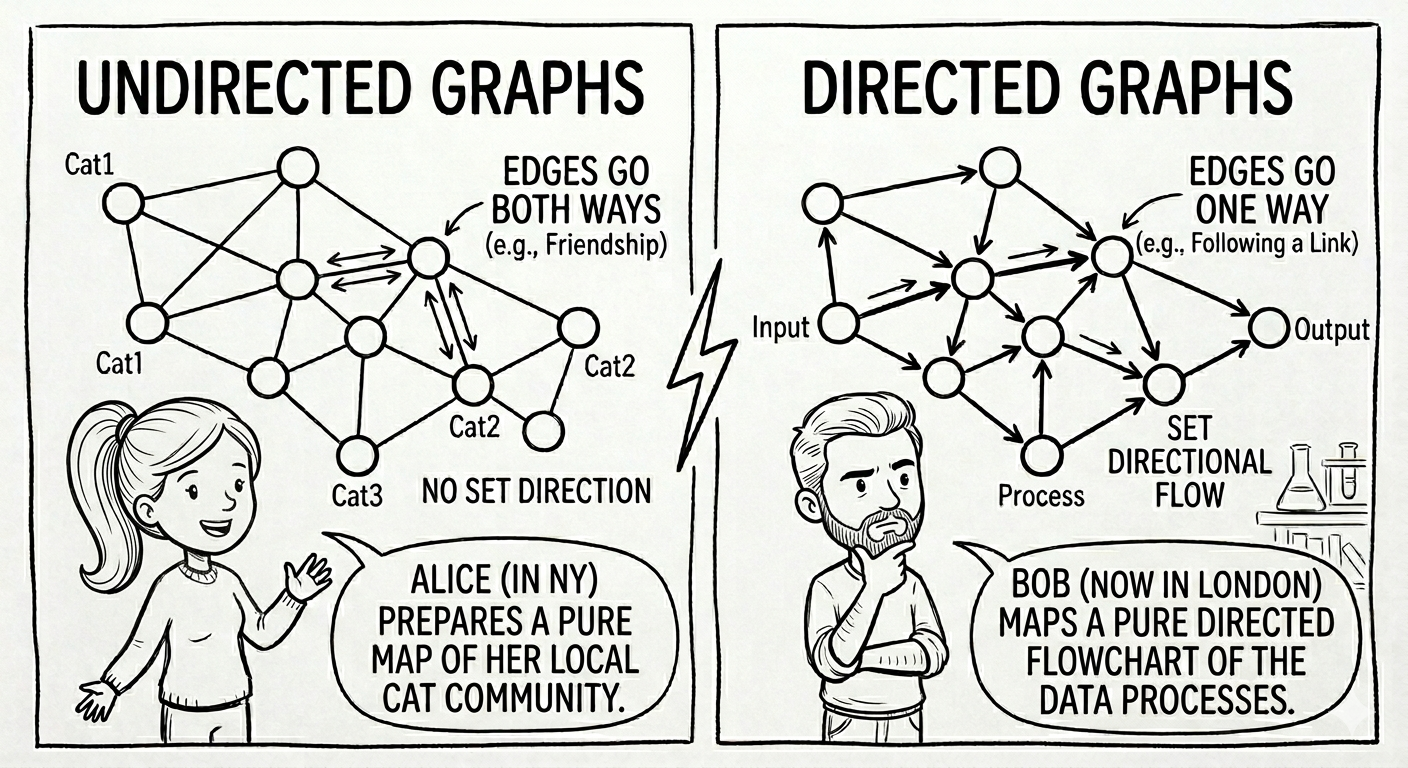
\includegraphics[width=0.8\textwidth]{figures/graph_theory.png}
    \caption{Alice and Bob have different graph. Alice has a undirected graph which means the edges can go both way. Bob has a directed graph, the relationship between two different nodes have been determined by the direction. Image is generated by Gemini.}
    \label{fig: graph_theory}
\end{figure}

So, graph states are a special class of multi-qubit quantum states that can represents graphs. In a graph state, each vertex (or node) corresponds to a qubit, and edges represent entanglement between the qubits. The structure of the graph encodes the pattern of entanglement in the state.

For example, consider a simple graph with three vertices connected in a line: A -> B -> C, as shown in Figure \ref{fig: graph_a}. The corresponding graph state can be constructed by applying controlled-Z (CZ) gates between the qubits corresponding to the connected vertices. The resulting state would be
\begin{equation}
  \ket{G} = CZ_{AB} CZ_{BC} \ket{+}_A \ket{+}_B \ket{+}_C
\end{equation}
where $\ket{+} = \frac{1}{\sqrt{2}}(\ket{0} + \ket{1})$ is the plus state. Then how about the graph state for the graph shown in Figure \ref{fig: graph_b}? The corresponding graph state can be constructed by applying controlled-Z (CZ) gates between the qubits corresponding to the connected vertices. The resulting state would be
\begin{equation}
  \ket{G} = CZ_{AB} CZ_{BC} CZ_{AC} CZ_{CD} \ket{+}_A \ket{+}_B \ket{+}_C \ket{+}_D
\end{equation}
Here, the controlled-Z gates are applied according to the edges in the graph: $CZ_{AB}$ for the edge between A and B, $CZ_{BC}$ for the edge between B and C, $CZ_{AC}$ for the edge between A and C, and $CZ_{CD}$ for the edge between C and D, and it can be written as
\begin{equation}
  \text{Controlled-Z}_{ij} = \ket{0}_i\bra{0} \otimes I_j + \ket{1}_i\bra{1} \otimes Z_j = \begin{bmatrix}
    1 & 0 & 0 & 0 \\
    0 & 1 & 0 & 0 \\
    0 & 0 & 1 & 0 \\
    0 & 0 & 0 & -1
  \end{bmatrix}
\end{equation}

\begin{figure}[htbp]
    \centering
    
    % === 图 A: 三节点横向排列 ===
    \begin{subfigure}[b]{0.45\textwidth}
        \centering
        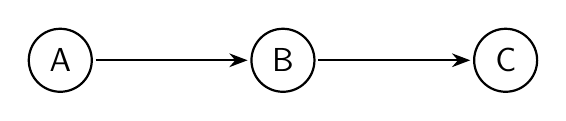
\begin{tikzpicture}[node distance=2cm] % 设置节点间的默认距离
            % 1. 定义节点位置
            \node[node_style] (A) {A};
            \node[node_style, right=of A] (B) {B}; % B 在 A 的右边
            \node[node_style, right=of B] (C) {C}; % C 在 B 的右边
            
            % 2. 绘制带箭头的连线
            \draw[arrow_style] (A) -- (B);
            \draw[arrow_style] (B) -- (C);
        \end{tikzpicture}
        \caption{Three-node Chain (A $\to$ B $\to$ C)}
        \label{fig: graph_a}
    \end{subfigure}
    \hfill % 在两个子图之间加入弹性间距
    % === 图 B: 四节点正方形排列 ===
    \begin{subfigure}[b]{0.45\textwidth}
        \centering
        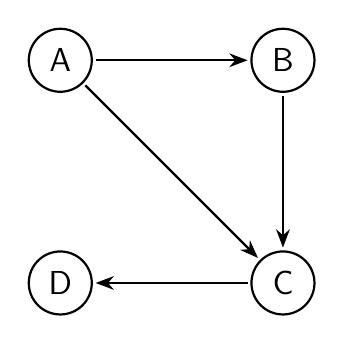
\begin{tikzpicture}[node distance=2cm]
            % 1. 定义节点位置 (正方形)
            \node[node_style] (A) {A};
            \node[node_style, right=of A] (B) {B};    % B 在 A 右边
            \node[node_style, below=of A] (D) {D};    % D 在 A 下边 (形成左侧边)
            \node[node_style, below=of B] (C) {C};    % C 在 B 下边 (形成右侧边)
            % 注意：这里的顺序保证了 ABCD 是顺时针或逆时针排列，
            % 我们通过 A->B 和 D->C 连线来控制箭头的逻辑。
            
            % 2. 绘制带箭头的连线
            \draw[arrow_style] (A) -- (B);            % A -> B
            \draw[arrow_style] (A) -- (C);            % A -> C (对角线)
            \draw[arrow_style] (B) -- (C);            % B -> C
            \draw[arrow_style] (C) -- (D);            % C -> D
        \end{tikzpicture}
        \caption{Four nodes in Square (A $\to$ B, A $\to$ C, B $\to$ C, C $\to$ D)}
        \label{fig: graph_b}
    \end{subfigure}
    
    \caption{Two different graph that can be converted to graph states.}
    \label{fig: two_graphs}
\end{figure}
Graph states are a powerful resource for quantum computing, as they can be used to implement various quantum algorithms and protocols. They also play a crucial role in the study of quantum entanglement and quantum correlations. Graph states provide a natural framework for optimization problems.

\begin{SBUBox}{$n$-Qubit Celebrity States}
  The GHZ State:
  \begin{equation*}
    \ket{\text{GHZ}_n} = \frac{1}{\sqrt{2}} \left( \ket{00\dots0} + \ket{11\dots1} \right)
  \end{equation*}
  This state is the $n$-qubit generalization of the Bell state $\ket{\Phi^+}$. 
  
  The W State:
  \begin{equation*}
    \ket{\text{W}_n} = \frac{1}{\sqrt{n}} \left( \ket{100\dots0} + \ket{010\dots0} + \dots + \ket{000\dots1} \right)
  \end{equation*}
  This state is a superposition of all possible states where exactly one qubit is in $\ket{1}$.
\end{SBUBox}


\newpage
\section{Rule No.1: Follow the Algorithms}










\end{document}
